\documentclass[11pt]{article}
\bibliographystyle{plain}
\usepackage{geometry} % see geometry.pdf on how to lay out the page. There's lots.
\usepackage{amsmath,amssymb} 
\usepackage{epsfig,epsf,subfigure}
\geometry{a4paper} 


%\documentclass{article}

\begin{document}
 
\LARGE
\begin{center}
TMA4280: Introduction to Supercomputing
\end{center}
\vspace{1in}

\begin{center}
{\bf Introduction}
\end{center}

\Large
\vspace{0.5in}
\begin{center}
January 2011
\end{center}

\vspace{0.5in}

\begin{center}
\copyright Einar M. R{\o}nquist \\
Department of Mathematical Sciences\\
NTNU, N-7491 Trondheim, Norway\\
All rights reserved \\
\ \\
Revised by Arne Morten Kvarving, December, 2011
\end{center}

\large

\newpage

\section{Supercomputing}

What do we mean by supercomputing? In general, we mean using computers
to solve problems which are very compute intensive, i.e., problems which require 
large computing resources in terms of memory or floating-point operations, or both. 
Examples of problems requiring supercomputing are weather forecasting
(met.no uses the supercomputing facility here at NTNU),
oil exploration (reservoir simulation), seismic analysis (an inverse problem), 
computational chemistry, computational physics, computational mechanics
(e.g., structural mechanics, fluid mechanics), and materials science. 

Due to the resource demanding aspects of supercomputing,  
it is important to make the whole solution process as efficient as possible.
Examples of important issues to study are: 
numerical/computational algorithms which are fast, robust and accurate,
the software development, treatment of large data sets, 
visualization, and validation of the simulation results. 

Supercomputing typically implies the use of parallel processing. 
This means that the underlying algorithms used need to be designed and tuned
for such a computing environment. The software development typically becomes more 
involved compared to a single-process implementation even though  the trend is to 
abstract the machine specific details as much as possible. 

Because of the compute-intensive (memory, floating-point, I/O) 
nature of these problems,
they often require special high-end computing platforms. In Norway, there is at least 
one such system at each major university. The large oil companies in Norway also have 
such computing platforms. Each system is still quite expensive to purchase, to operate
and to maintain. In addition, often special intrastructure needs to be built around such 
systems: special rooms (security), power supply, cooling systems etc. 
Due to the overall investment, both in terms hardware and in terms of human resources, 
it is important to use these systems as efficiently as possible
(each system typically lasts only a few years). 

Even if the current systems are powerful, it is important to make progress in terms 
of making such systems easier to build and to use, and to develop more 
efficient computational algorithms. This will enable larger and more realistic problems 
to be simulated, which translates into progress in science and engineering 
(which are the "classical" applications for supercomputing), but also in 
other emerging areas such as the medical field. 


In the following, let us briefly mention some of the issues involved when working with 
 a specific application. Assume that we have a program for simulating the blood flow 
through part of a vein. Let $T_1$ be the solution time on a single processor
(in reality, such a simulation would probably not fit on a single-processor machine). 

Assume now that we port this simulation to a multi-processor 
system with $P$ processors. 
Ideally, we would like the solution time to be reduced by a factor of $P$. 
Another way of saying this is that we would like to achieve a speedup 
\begin{align}
S_p=T_1/T_p = P,
\end{align} 
where $T_p$ is the solution time on $P$ processors. 
Typically, the speedup $S_p < P$. As we increase the number of processors to solve
our particular (fixed) problem, we will first see a good speedup, followed by a 
degradation as we add more and more processors. The main explanation for this is easy 
to understand. In order to achieve a perfect speedup, we cannot have any overhead
when moving from a single processor system to a multi-processor system. 
In reality, we have communication between the processors. 
As the number of processors is increased, the work per processor goes down, while 
the overall communication (overhead) goes up. A critical issue is therefore to 
minimize the communication overhead so that we can take advantage of larger systems
for a fixed problem. 

We should here remark that one of the major advantages of having access to a 
supercomputing facility is the possibility to solve much larger problems than what 
is possible on a smaller system. Hence, as we increase the number of processors, 
we may also increase the problem size so that the work per processor remains fixed. 
We will consider some of these issues in this course. 


Let us now discuss the single-processor performance a bit more. 
Assume for the moment that we have two different versions (executables), $A$ and $B$,
of the particular application. We also assume that the underlying numerical algorithms
are identical. The simulation times for the two versions are 
denoted as $T_1^A$ and $T_1^B$, respectively. We observe that 
\begin{align}
T_1^A = 3 T_1^B.
\end{align} 

Why are the two simulation times so different since the numerical algorithms are the same?

\begin{figure}[htbp]
  \begin{center}
    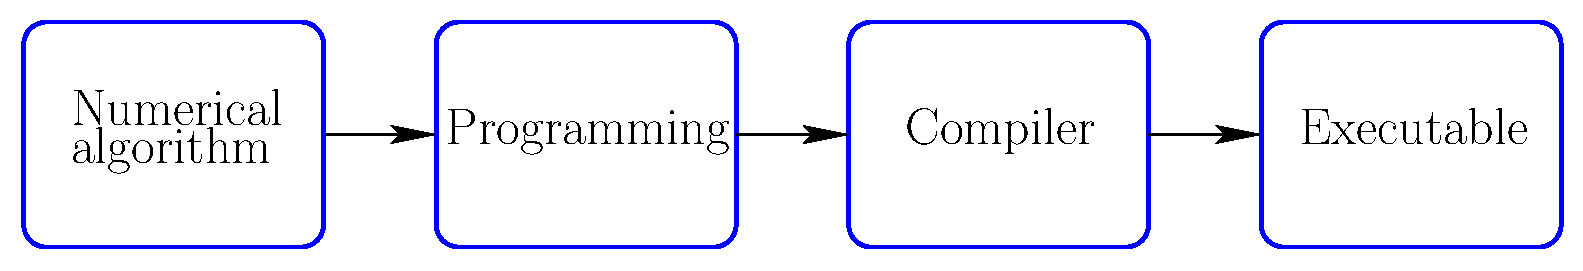
\includegraphics[scale=0.5]{figure1}
  \end{center}
\caption{
}
\label{fig:single}
\end{figure}

We only mention a few aspects which may have caused this; see Figure \ref{fig:single}: 
\begin{itemize}
\item different choice of data structure /  memory layout during the programming;
\item different use of optimized numerical libraries;
\item different choices of compiler optimization.
\end{itemize}
We will look at some of these issues in this course. 
Note that it is typically harder to achieve a good speedup for version B compared to 
version A, even though $T_1^B  < T_1^A$ (can you suggest a reason why?). 

Are there other ways to change the solution time for our particular simulation?
Yes; we mention two distinct ways: 
\begin{itemize}
\item change the computer; 
\item change the computational / numerical algorithms. 
\end{itemize}
Progress in the available hardware has been impressive over the past decades. 
However, it is important to realize that progress in computational algorithms has
been equally impressive. Note that developing a new algorithm which 
requires only half the number of floating point operations is 
equally important as buying a new computer with twice the performance
in terms of floating point operations per second (FLOPS). 

We will discuss a few selected numerical algorithms in this course, e.g., 
numerical solution of partial differential equations (primarily finite difference methods), 
iterative and direct methods for solving linear systems of equations, 
basic linear algebra routines, and a little bit about statistical methods (Monte Carlo methods). 

\newpage

\section{Floating point representation}

This section gives a brief introduction to the IEEE standard
(IEEE-754) for floating point representation. 
A basic understanding of the standard is appropriate given 
the importance of floating point operations in this course. 

All real numbers are represented with a finite number of bits. 
The representation is depicted in Figure \ref{fig:fp}.
The sign bit is certainly easy to understand. A value $S=0$ means that the number is
positive, while a value $S=1$ means that the number is negative. 


\begin{figure}[htbp]
  \begin{center}
    \includegraphics[scale=1]{ieee}
  \end{center}
  \caption{Each floating point has a binary representation with 
three fields: $S$ denotes the sign of the number, 
$E$ is an exponent, and $F$ is the fraction part of the mantissa.
}
\label{fig:fp}
\end{figure}


The actual decimal value $V$ of the floating point is
\begin{eqnarray}
V = (-1)^S \cdot 2^{E-B}\cdot M
\end{eqnarray}
where $M$ is the mantissa (here in decimal representation) and 
$B$ is denoted as the {\em bias} which will be explained below.
The exponent E is always adjusted such that the mantissa can be expressed as 
\begin{eqnarray}
M = \underbrace{1}_{\times2^0}.\overbrace{\underbrace{b_1}_{\times2^{-1}}\underbrace{b_2}_{\times2^{-2}}...}^{F}
\end{eqnarray}
where $F$ denotes the fraction of the mantissa in binary
representation (i.e., the binary digits $b_1b_2...$). 
Since this representation is always
assumed, the binary number 1 in the front is not explicitly
represented. Note that, in decimal representation, 
\begin{eqnarray}
1\leq M <  2 \quad 
\end{eqnarray}
since the fraction $F$ in decimal representation is always less then one. 

There are many more details regarding floating point representation. 
For example, the implicitly assumed binary number 1 in the mantissa
is only true for what is referred to as {\em normalized} numbers. 

\begin{center}
{\bf Table 1} \\
Number of bits for common floating point precisions
\end{center}
\begin{center}
\begin{tabular}{|c|c|c|c|c|c|c|c|} \hline
Precision & $S$ & $E$ & $F$ & Total  
  \\ \hline
Single & $1$ & $8$ & $23$ & 32  
  \\ \hline
Double & $1$ & $11$ & $52$ & 64 
  \\ \hline
\end{tabular}
\end{center}

A few words about the exponent $E$. In single precision, $E$ is
represented using 8 bits, giving 256 possibilities, of which 
254 are used to represent normalized numbers. 
The values $E=0$ and $E=255$ are primarily reserved for zero and
infinities. 
The actual exponent used to find the corresponding decimal value 
of a normalized number is $E-B$; see equation (1). 
For single precision, $B=127$. 

We can now compute the maximum 
and minimum numbers that we can represent in single precision (i.e.,
using 32 bits):
\begin{eqnarray}
V_{max} &=& 1\cdot 2^{254-127}\cdot 2 = 3.40\ldots 10^{38} 
\label{maxnumber}\\
V_{min} &=& 1\cdot 2^{1-127}\cdot 1 = 2^{-126} = 1.17\ldots 10^{-38}
\label{minnumber}
\end{eqnarray}
As we can see, this is a significant range. 

Having considered the range, let us now consider the accuracy of a 
given floating point number. Again, consider the single precision
case. The fraction of the mantissa is represented using 23 bits, 
meaning that the smallest {\em fraction} that can be represented is 
\begin{eqnarray*}
2^{-23} = 1.19\ldots 10^{-7} \quad .
\end{eqnarray*}
This implies that {\em any} floating point number using single precision 
(covering the whole range discussed above) have about 7 digits of
accuracy. 

\vspace{.2in}
\noindent {\bf Exercise 1}. Consider the maximum and minimum numbers 
derived in (\ref{maxnumber})-(\ref{minnumber}). How many digits should we include in each
of these numbers?\\
\\
\noindent {\bf Exercise 2}. Find the binary floating point
representation of the decimal number 4.25 in single precision.\\
\\
\noindent {\bf Exercise 3}. How many digits of accuracy does a 
floating point number in double precision have? 

\section{Integer representation}

An integer is typically represented using 32 bits. One bit is used to represent the sign. 
Hence, the possible integers will be in the range 
$\pm 2^{31} \approx \pm \, 2\cdot 10^9$.

If an algorithm includes a loop which needs to be done $n$ times (e.g., a Monte Carlo
simulation), $n$ needs to be less than approximately $10^9$. This may seem 
sufficient, however, there could be situations when this limitation could become an issue. 

\vspace{.2in}
\noindent {\bf Exercise 4}. Propose a way to avoid the above limitation. 

\newpage
\section{Floating point performance}

The basic operations of adding, multiplying, subtracting and dividing 
two floating point numbers are counted as floating point operations. 

Floating point performance is usually measured in number of floating point 
operations per second, commonly abbreviated as FLOPS; for a brief discussion,
see \texttt{http://en.wikipedia.org/wiki/FLOPS}.

Since current computer systems
typically perform many of these operations per seconds, abbreviations like MFLOPS 
(megaflops), GFLOPS (gigaflops), TFLOPS (teraflops), and PFLOPS (petaflops)
are common to use. 

When we speak about the speed of a computer, we will typically mean 
the floating point performance.   

\vspace{.2in}
\noindent {\bf Exercise 5}. Let $c$ be a scalar (a floating point number), 
let $\underline{x}$, $\underline{y}$, and $\underline{z}$
be vectors, each comprising $n$ floating point numbers, and let 
$\underline{A}$ be an $n\times n$ matrix. 
How many floating point operations does it take to perform the following 
basic linear algebra operations: $\underline{z} = \underline{x} +  c \underline{y}$?
What about the matrix-vector product $\underline{y} = \underline{A}\,\underline{x}$ ?\\


\clearpage
\section{Storage requirement}

It is quite common today to do all the necessary computations using double precision. 
This means that 64 bits are used to represent each floating point number, which 
is equivalent to 8 bytes (8 bits per byte). 

Let us now consider how many floating point numbers we can store in the memory 
associated with a typical processor. Assume that we have available 4 Gbytes ($4\cdot 10^9$ bytes)
of main memory (or RAM: Random Access Memory); this is a quite typical size nowadays. 
This amount of memory is sufficient to represent a total of 512 millon 
floating point numbers in double precision. 

In practice, we could never use the entire memory for such a purpose. 
We also need space for our simulation program (instructions etc.). 
However, it gives an indication of the order of magnitude that we can handle. 

If we are solving differential equations or some other problem, we also need 
to use memory to store matrices, temporary variables, etc. 
The available memory to store the actual solution depends on the 
numerical algorithm, however, even a fairly scalable algorithm would typically 
only be able to handle a few million unknowns. 
Many algorithms would allow far fewer unknowns. 

Problems in science and engineering can easily require many million unknowns, 
perhaps even billions of unknowns. In order to solve such problems, 
we obviously need both more memory and increased computing power. 
This is achieved using parallel processing where multiple processors
(and memory modules), are connected into a single computational platform. 

\vspace{.2in}
\noindent {\bf Exercise 6}. Let $\underline{A}$ be an $n\times n$ matrix, 
and $\underline{x}$ and $\underline{b}$ be two vectors of length $n$. 
Assume that we want to solve the linear system of equations
\begin{align}
\underline{A}\,\underline{x} = \underline{b} 
\end{align}
using Gaussian elimination. Assume further 
that the matrix $\underline{A}$ is dense, meaning that 
we need to store all the $n^2$ entries in the matrix. 

What is (approximately) the largest equation system we can solve 
(i.e., the  largest number of $n$ we can use) and still be able 
to fit the whole problem in the main memory, which we assume is 1 Gbyte?

\newpage
\section{Past, current and future supercomputers}

Figure \ref{fig:perform_dev} and 
Figure \ref{fig:proj_perform_dev} depict the past and future 
performance development of the 500 fastest supercomputers in the world. 
More information about the top 500 systems can be found on 
\texttt{http://www.top500.org}. 

\vspace{2cm}
\begin{figure}[!ht]
  \centering
  \includegraphics[width=14cm]{Performance_Development}
  \caption{The figure shows the performance development since 1993 
for the top 500 supercomputers in the world. In particular, the figure indicates the 
performance development for the fastest system (number 1), 
the slowest system (number 500), and the sum of all the 500 fastest systems. }
  \label{fig:perform_dev}
\end{figure}
\vspace{1cm}

\begin{figure}[!ht]
  \centering
  \includegraphics[width=14cm]{Projected_Performance_Development}
  \caption{The figure shows the projected performance development assuming that the past trends continues. 
 }
  \label{fig:proj_perform_dev}
\end{figure}

\clearpage

\begin{table}
\caption{Supercomputers at NTH/NTNU�}
\centering
\begin{tabular}{|l|l|l|l|l|l|}
\hline
Year & System & \#proc & type & GF (*)\\
\hline
1986-1992 & Cray X-MP & 2 & vector & 0.5 \\
1992-1996 & Cray Y-MP & 4 & vector & 1.3\\
1995-2003 & Cray J90     & 8 & vector & 1.6 \\
1992-1999 & Intel Paragon & 56 & MPP & 5.0\\
1996-2003 & Cray T3E & 96 & MPP & 58\\
2000-2001 & SGI O2 & 160 & CCNUMA & 100\\
2001-2008 & SGI O3 & 898 & CCNUMA & 1000\\
2006-2011 & IBM P5+ & 2976 & distributed SMP & 23500\\
2012-     & SGI Altix ICE X & 23040 & distributed SMP & 497230 \\
\hline
\end{tabular}
\label{tab:history_ntnu}
\end{table}
%\noindent(*)   several upgrades; currently 512 processors left\\
(*) maximum theoretical performance in Gflops

\vspace{.3in}
In 1986 a supercomputing center was established at NTH. 
Table \ref{tab:history_ntnu} gives a summary of the supercomputers
at NTH/NTNU since then. 

\it NOTE: Some of this information is guesswork as the machine was not available at
when revising this document. \rm
The current supercomputer at NTNU is an SGI Altix system with 20736 (physical)
processors. For an example of what such a system looks like, see Figure \ref{fig:njord_2} and \ref{fig:njord_1}.
Some of the exercises in this course will be done using this system.
Some of the key characteristics of this system are: 

\begin{itemize}
\item Full name: \texttt{vilje.hpc.ntnu.no}
\item System: SGI Altix ICE
\item Type: distributed SMP 
\item Number of nodes: 1440
\item A single node: \\
a shared memory system; 2 octa-core chips; 32 GB memory
\item Number of cores (processors): 23040
\item CPU type: Intel Sandy Bridge
\item Theoretical total peak: 479.23 Tflops
\item Weight: This machine is shy and refuse to tell me.
\end{itemize}



\begin{figure}[!ht]
  \centering
  \includegraphics[width=8cm]{njord_2}
  \caption{A photo of \texttt{njord}, the previous IBM supercomputer system at NTNU. 
  Courtesy of Arve Dispen. }
  \label{fig:njord_2}
\end{figure}

\begin{figure}[!ht]
  \centering
  \includegraphics[width=8cm]{njord_1}
  \caption{A photo of \texttt{njord}, the previous IBM supercomputer system at NTNU. 
  Courtesy of Arve Dispen. }
  \label{fig:njord_1}
\end{figure}

\newpage
\section{Applications}

\vspace{2cm}
\begin{figure}[!ht]
  \centering
  \includegraphics[width=12cm]{met}
  \caption{Example of use of supercomputing: weather forecasting. The Meteorological Institute in Norway uses the supercomputer \texttt{njord} every day. 
  Source: \texttt{http://met.no}.}
  \label{fig:met}
\end{figure}

\begin{figure}[!ht]
  \centering
  \includegraphics[width=8cm]{climate_model}
  \caption{Example of use of supercomputing: climate modelling. 
  For more information, see 
  \texttt{http://www.bcm.uib.no} (Bergen Climate Model) and 
\texttt{http://www.bjerknes.uib.no} (Bjerknes Centre for Climate Research).}
  \label{fig:climate}
\end{figure}

\end{document}
